\documentclass{standalone}
\usepackage{tikz}
\begin{document}
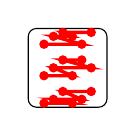
\begin{tikzpicture}[scale=1.0]
  % draw rounded cell boxes
  \draw[rounded corners=3pt] (0,0) rectangle (1,1);
  \fill[red] (0.2,0.05) circle (0.06);
  \fill[red] (0.32,0.1) circle (0.06);
  \fill[red] (0.44,0.2) circle (0.06);
  \fill[red] (0.56,0.05) circle (0.06);
  \fill[red] (0.6799999999999999,0.1) circle (0.06);
  \fill[red] (0.8,0.2) circle (0.06);
  \draw[red, line width=1.2pt] (0.2,0.05) -- (0.56,0.05) -- (0.32,0.1) -- (0.6799999999999999,0.1) -- (0.44,0.2) -- (0.8,0.2);
  \fill[red] (0.2,0.4) circle (0.06);
  \fill[red] (0.32,0.5) circle (0.06);
  \fill[red] (0.44,0.6000000000000001) circle (0.06);
  \fill[red] (0.56,0.4) circle (0.06);
  \fill[red] (0.6799999999999999,0.6000000000000001) circle (0.06);
  \fill[red] (0.8,0.5) circle (0.06);
  \draw[red, line width=1.2pt] (0.2,0.4) -- (0.56,0.4) -- (0.32,0.5) -- (0.8,0.5) -- (0.44,0.6000000000000001) -- (0.6799999999999999,0.6000000000000001);
  \fill[red] (0.2,0.8) circle (0.06);
  \fill[red] (0.32,0.9) circle (0.06);
  \fill[red] (0.44,0.95) circle (0.06);
  \fill[red] (0.56,0.9) circle (0.06);
  \fill[red] (0.6799999999999999,0.8) circle (0.06);
  \fill[red] (0.8,0.95) circle (0.06);
  \draw[red, line width=1.2pt] (0.2,0.8) -- (0.6799999999999999,0.8) -- (0.32,0.9) -- (0.56,0.9) -- (0.44,0.95) -- (0.8,0.95);
\end{tikzpicture}
\end{document}